%\documentclass[12pt]{article}

\questionheader{ex:s2.2}

%%%%%%%%%%%%%%%%%%
%\subsection*{\Conceptual}
%%%%%%%%%%%%%%%%%%


\begin{question}
Suppose that the vector field $\vv(x,y)$ sketched below represents the velocity of 
moving water at the point $(x,y)$ in the first quadrant of the $xy$-plane.
  \begin{center}
       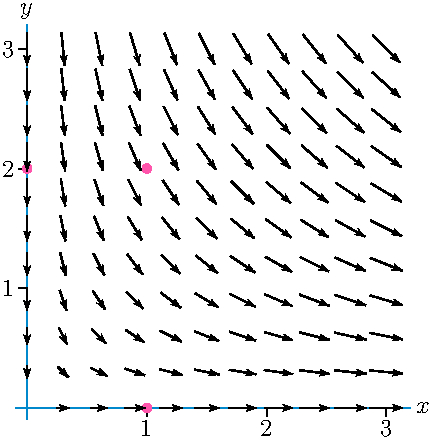
\includegraphics{duckyField.pdf}
  \end{center}
Sketch the path followed by a rubber ducky dropped in at the point
\begin{enumerate}[(a)]
\item $(0,2)$
\item $(1,0)$
\item $(1,2)$
\end{enumerate}
%Describe its velocity as it changes position.
\end{question}

%\begin{hint} 
%\end{hint}

\begin{answer} 
\begin{center}
       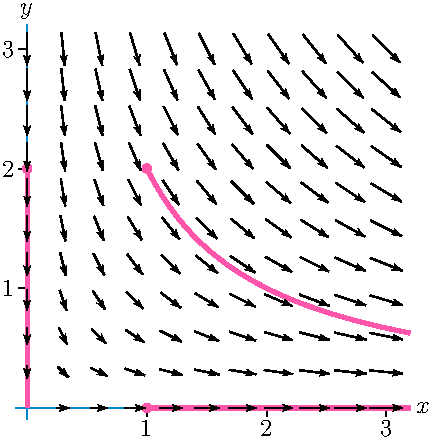
\includegraphics{duckyField2.pdf}
  \end{center}
\end{answer}

\begin{solution}
(a) At every point of the positive $y$-axis, the velocity vector $\vv(0,y)$
points straight down. So a rubber ducky placed in the water at $(0,2)$
just floats straight down the positive $y$-axis towards the origin.

\begin{center}
       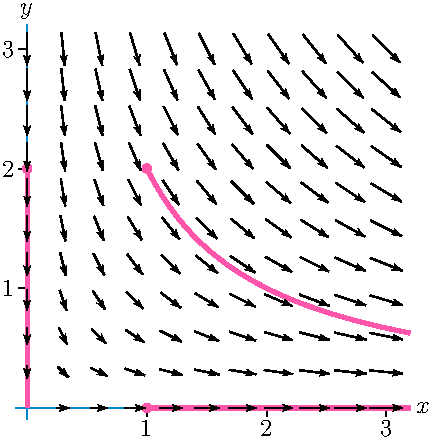
\includegraphics{duckyField2.pdf}
  \end{center}

\noindent
(b) At every point of the positive $x$-axis, the velocity vector $\vv(x,0)$
points straight to the right. So a rubber ducky placed in the water at $(1,0)$
just floats rightward along the positive $x$-axis.

\noindent
(c) At every point of the first quadrant away from the axes, the 
velocity vector $\vv(x,y)$ points downwards and towards the right. So a 
rubber ducky placed in the water at $(1,2)$ always floats down and to 
the right. The closer the ducky gets to the $x$--axis the more rightward 
its motion becomes. 

\end{solution}


\begin{question}
Find a vector field $\vv(x,y)$ for which
\begin{align*}
x(t) &= e^{-t}\cos t \\
y(t) &= e^{-t}\sin t \\
\end{align*}
is a field line.
\end{question}

\begin{hint} 
Express $x'(t)$ and $y'(t)$ purely in terms of $x(t)$ and $y(t)$.
\end{hint}

\begin{answer} 
$\vv(x,y) = (-x-y\,,\,x-y)$
\end{answer}

\begin{solution}
The derivatives
\begin{alignat*}{3}
x'(t) &= -e^{-t}\cos t - e^{-t}\sin t &&= -x(t)-y(t) \\
y'(t) &= -e^{-t}\sin t + e^{-t}\cos t &&= -y(t)+x(t) 
\end{alignat*}
So $\big(x(t),y(t)\big)$ is a solution of the system of differential equations
\begin{align*}
\diff{x}{t} &= v_1(x,y) = -x-y \\
\diff{y}{t} &= v_2(x,y) = \phantom{-}x-y
\end{align*}
So the vector field is $\vv(x,y) = \big(v_1(x,y)\,,\,v_2(x,y)\big) 
                                 = (-x-y\,,\,x-y)$.
\end{solution}




%\begin{question}
%The direction field shown below represents the differential equation blah. If the initial condition is $y=blah$, what is $\lim\limits_{t \to \infty} y$?
%\end{question}
%
%\begin{hint} 
%\end{hint}
%
%\begin{answer} 
%\end{answer}
%
%\begin{solution}
%\end{solution}



%%%%%%%%%%%%%%%%%%
\subsection*{\Procedural}
%%%%%%%%%%%%%%%%%%

\begin{question}[M317 2010A] %1
Consider the function $f(x,y) = xy$.
\begin{enumerate}[(a)]
\item
Explicitly determine the field lines (flow lines) of 
$\vF(x,y) = \vnabla f$.
\item
Sketch the field lines of $\vF$ and the level curves of $f$ in the same diagram.
\end{enumerate}
\end{question}

\begin{hint} 
Review \S\eref{CLP317}{sec:fieldLines} in the CLP-4 text.
\end{hint}

\begin{answer} 
(a) $\frac{x^2}{2} =\frac{y^2}{2} +C$

(b) 
  \begin{center}
       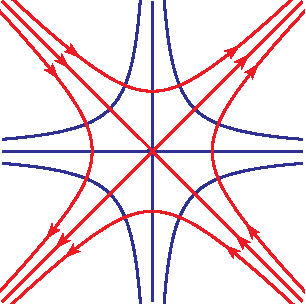
\includegraphics{OE10A_1.pdf}
  \end{center}

\end{answer}

\begin{solution} (a) The field lines of $\vF(x,y) = \vnabla f
=y\,\hi + x\,\hj$ obey
\begin{align*}
\frac{\dee{x}}{y} = \frac{\dee{y}}{x}
\iff x\,\dee{x} = y\,\dee{y}
\iff \frac{x^2}{2} =\frac{y^2}{2} +C
\end{align*}
for any constant $C$.

\noindent (b)
The sign data
\begin{align*}
\hi\cdot\vF(x,y) = y
    \left.\begin{cases}
             >0 &\text{if $y>0$} \\
             =0 &\text{if $y=0$} \\
             <0 &\text{if $y<0$} 
       \end{cases}\right\}\qquad
\hj\cdot\vF(x,y) = x
    \left.\begin{cases}
             >0 &\text{if $x>0$} \\
             =0 &\text{if $x=0$} \\
             <0 &\text{if $x<0$} 
       \end{cases}\right\}\qquad
\end{align*}
is visually displayed in the figure on the left below. The arrows in the
figure on the left gives us the direction of motion along 
the field lines $\frac{x^2}{2} =\frac{y^2}{2} +C$ (in red) in the 
figure on the right below. Some equipotential curves $xy=C$ are 
also sketched (in blue) in the figure on the right below.

  \begin{center}
       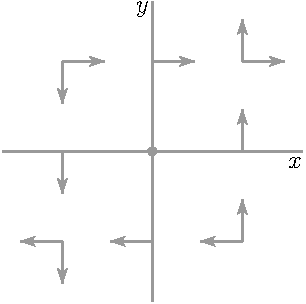
\includegraphics{OE10A_1Sign.pdf}\qquad\qquad
       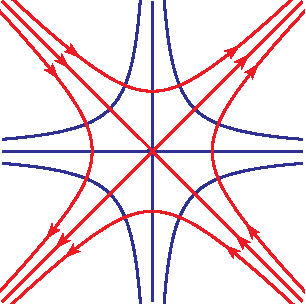
\includegraphics{OE10A_1.pdf}
  \end{center}


\end{solution}

%%%%%%%%%%%%%%%%%%%%%%%%%%%
\begin{question}[M317 2003A] %1
Find the field line of the vector field
$\vF= 2y\,\hi+ \frac{x}{y^2}\,\hj+e^y\hk$ that passes through
$(1,1,e)$.
\end{question}

%\begin{hint} 
%\end{hint}

\begin{answer} 
$x=y^2$, $z=e^y$
\end{answer}

\begin{solution} 
The field lines obey
\begin{equation*}
\frac{\dee{x}}{2y}=\frac{\dee{y}}{x/y^2}=\frac{\dee{z}}{e^y}
\qquad\text{ if $x,y\ne 0$}
\end{equation*}
In particular
\begin{align*}
\frac{\dee{x}}{2y}=\frac{y^2\,\dee{y}}{x}
\implies
x\,\dee{x}=2y^3\,\dee{y}
\implies
\frac{1}{2}x^2=\frac{1}{2}y^4+C
\end{align*}
Since $y=1$ when $x=1$, $C=0$. So $x=y^2$ and
\begin{equation*}
\frac{\dee{y}}{x/y^2}=\frac{\dee{z}}{e^y}
\implies
e^ydy=dz
\implies
z=e^y+D
\end{equation*}
Since $z=e$ when $y=1$, $D=0$. So the field line is
\begin{equation*}
x=y^2 \qquad z=e^y
\end{equation*}
\end{solution}

%%%%%%%%%%%%%%%%%%%%%%%%%%%
\begin{question}[M317 2001A] %1
 Find and sketch the field lines of the vector field
$\vF= x\,\hi+ 3y\,\hj$.
\end{question}

%\begin{hint} 
%\end{hint}

\begin{answer}
The field lines are $y=C'x^3$ with $C'$ a nonzero constant,
as well as $x=0$ and $y=0$.

\begin{center}
   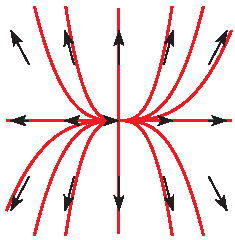
\includegraphics{fline.pdf}
\end{center}

\end{answer}

\begin{solution} 
 The field lines obey
\begin{align*}
&\frac{\dee{x}}{x}=\frac{\dee{y}}{3y}\qquad\text{ if $x,y\ne 0$}\\
&\implies 3\ln |x|=\ln |y|+C\\
&\implies |x|^3=e^C|y| \\
&\implies y=\pm e^{-C}x^3 \\
&\implies y=C'x^3
\end{align*}
with $C'$ a nonzero constant.
$x=0$ and $y=0$ are also field lines,
since on the $y$-axis $\vF\parallel\hj$ and
on the $x$-axis $\vF\parallel\hi$.

\begin{center}
   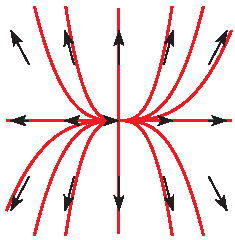
\includegraphics{fline.pdf}
\end{center}
\end{solution}




%%%%%%%%%%%%%%%%%%
%\subsection*{\Application}
%%%%%%%%%%%%%%%%%%

